\documentclass[12pt,a4paper,oneside]{report}
\usepackage[utf8]{inputenc}
\usepackage[english,russian]{babel}
\usepackage{amsmath}
\usepackage{amssymb}
\usepackage{geometry}
\usepackage{sverb}
\usepackage{graphicx}
\usepackage{pdfpages}
\usepackage{hyperref} 
\usepackage{url}
\usepackage{titlesec, blindtext, color}
\usepackage{listings}
\usepackage{pgfplots}
\pgfplotsset{compat=newest}
\graphicspath{{../}}
\DeclareGraphicsExtensions{.pdf,.png,.jpg}
\usepackage{tabularx}
\usepackage{subcaption}
\usepackage{colortbl}
\usepackage{multirow}
\usepackage{longtable}
\usepackage{enumitem}
\usepackage{algorithm}
\usepackage{tikz}
\usepackage[noend]{algpseudocode}
\usepackage{float}
\definecolor{gray75}{gray}{0.75}
\definecolor{Blue}{HTML}{5D8AA8}
\newcommand{\hsp}{\hspace{20pt}}

\newcommand{\RomanNumeralCaps}[1]
{\MakeUppercase{\romannumeral #1}}



% Для листинга кода:
\lstset{ %
	language=c,                 % выбор языка для подсветки (здесь это С)
	basicstyle=\small\sffamily, % размер и начертание шрифта для подсветки кода             % где поставить нумерацию строк (слева\справа)
	numberstyle=\tiny,           % размер шрифта для номеров строк
	stepnumber=1, 
	keywordstyle=\color{blue},% размер шага между двумя номерами строк
	numbersep=5pt,                % как далеко отстоят номера строк от подсвечиваемого кода
	showspaces=false,            % показывать или нет пробелы специальными отступами
	showstringspaces=false,      % показывать или нет пробелы в строках
	showtabs=false,             % показывать или нет табуляцию в строках
	frame=single,              % рисовать рамку вокруг кода
	tabsize=2,                 % размер табуляции по умолчанию равен 2 пробелам
	captionpos=t,              % позиция заголовка вверху [t] или внизу [b] 
	breaklines=true,           % автоматически переносить строки (да\нет)
	breakatwhitespace=false, % переносить строки только если есть пробел
	escapeinside={\#*}{*)}  % Стиль литералов
}


\titleformat{\chapter}[hang]{\Huge\bfseries}{\thechapter.\textcolor{gray75}\hsp}{0pt}{\Huge\bfseries}
\newcommand{\specchapter}[1]{\chapter*{#1}\addcontentsline{toc}{chapter}{#1}}
\newcommand{\specsection}[1]{\section*{#1}\addcontentsline{toc}{section}{#1}}
\newcommand{\specsubsection}[1]{\subsection*{#1}\addcontentsline{toc}{subsection}{#1}}

% геометрия


\setcounter{tocdepth}{4} % фикс переноса 
\righthyphenmin = 2
\tolerance = 2048


\thispagestyle{empty}

\geometry{pdftex, left = 3cm, right = 1cm, top = 2cm, bottom = 2cm}

\begin{document}

\thispagestyle{empty}

\thispagestyle{empty}
\noindent \begin{minipage}{0.15\textwidth}
	
\includegraphics[width=\linewidth]{b_logo}
\end{minipage}
\noindent\begin{minipage}{0.9\textwidth}\centering
	\textbf{Министерство науки и высшего образования Российской Федерации}\\
	\textbf{Федеральное государственное бюджетное образовательное учреждение высшего образования}\\
	\textbf{«Московский государственный технический университет имени Н.Э.~Баумана}\\
	\textbf{(национальный исследовательский университет)»}\\
	\textbf{(МГТУ им. Н.Э.~Баумана)}
\end{minipage}
\noindent\rule{18cm}{3pt}
\newline\newline
\noindent ФАКУЛЬТЕТ $\underline{\textbf{«ИНФОРМАТИКА И СИСТЕМЫ УПРАВЛЕНИЯ»}}$ \newline\newline
\noindent КАФЕДРА $\underline{\textbf{«ПРОГРАММНОЕ ОБЕСПЕЧЕНИЕ ЭВМ И ИНФОРМАЦИОННЫЕ}}$\newline\newline $\underline{\textbf{ТЕХНОЛОГИИ»(ИУ7)}}$\newline\newline
\noindent НАПРАВЛЕНИЕ ПОДГОТОВКИ $\underline{\textbf{09.03.04 ПРОГРАММНАЯ ИНЖЕНЕРИЯ}}$\newline\newline\newline\newline\newline\newline\newline
\begin{center}
    \begin{flushright}
    \Large\textbf{ОТЧЕТ}\newline
	\Large\textbf{по лабораторной работе № 3}\newline
	\end{flushright}
\end{center}
\noindent\textbf{Название:} $\underline{\text{Генерация случайных чисел}}$\newline\newline
\noindent\textbf{Дисциплина:} $\underline{\text{Моделирование}}$\newline\newline\newline\newline\newline\newline\newline\newline
\begin{tabular}{lcp{5em}lp{2em}l}
	\noindent\textbf{Студент} &  $\underline{\text{ИУ7-71Б~~}}$ &             &\hspace{1cm} & & $\underline{\text{В.С.Плотников}}$ \\\cline{4-3}
	 & (Группа) & &(Подпись,дата)  & & (И.О.Фамилия) \\
	 & & & & &\\
	\noindent\textbf{Преподаватель} &  & &\hspace{1cm} & &$\underline{\text{И.В.Рудаков ~~~~}}$ \\\cline{4-3} 
	 &  & & (Подпись,дата)  & &(И.О.Фамилия) \\
    \end{tabular}
\begin{center}
	\vfill
	Москва, \the\year
\end{center}
\clearpage



\section*{Задание}
\quad Необходимо изучить методы генерации псевдослучайных чисел и критерии оценки случайности последовательности. Надо реализовать критерий оценки случайной последовательностии сравнить результаты работы данного критерия на одноразрядных, двухразрядных и трехразрядных последовательностях целых чисел. Последовательности нужно получать алгоритмическим и табличным способами.

\section*{Способы получения последовательностей случайных чисел}
\quad Выделяют 3 основных способа:
\begin{enumerate}
    \item Аппаратный - случайные числа вырабатываются специальной электронной приставкой, то есть генератором случайных чисел. Как правило это практически любое внешнее устройство компьютера. Реализация этого способа не требует дополнительных вычислительных операций по выработке чисел, а необходима только операция обращения к этому внешнему устройству. Физическая основа - как правило шум на проводниковых и полупроводниковых приборах. Состоит из:
    \begin{itemize}
        \item Источник шума
        \item Ключевая схема
        \item Формировщик импульсов
        \item Пересчётная схема
    \end{itemize}
    Тогда случайное число как разница между соседним и предыдущем временем.

    \item Табличный (файловый) - формируется таблица и записывается в память. Математики проверили её на случайность и мы можем многократно её использовать. Недостаток - количество чисел ограничено.

    \item Алгоритмический (программный) - масса достоинств, однократная проверка, можно многократно воспроизводить последовательность, относительно малое место в оперативной памяти, не используются внешние устройства. Недостаток - запас чисел ограничен периодом, требуются затраты машинного времени.
\end{enumerate}

\section*{Линейный конгруэнтный метод}
\quad В данной работе был выбран линейный конгруэнтный метод в качестве алгоритмического.
Для осуществления генерации чисел данным методом, необходимо задать 4 числа:

\begin{center}
m > 0, модуль\\
0 $\leq$ a	$\leq$ m, \text{множитель}\\
0 $\leq$ c $\leq$ m, \text{приращение}\\
0 $\leq$ $X_0$ $\leq$ m, \text{начальное число}\\
\end{center}

Последовательность случайных чисел генерируется при помощи формулы:
\begin{equation}
X_{n+1}=(aX_n+c)\mod m
\end{equation}

\section*{Критерий $\chi^2$}
\quad Для выполнения работы был выбран критерий $\chi^2$. Это один из самых известных статистических критериев,  также это основной метод, используемый в сочетании с дргуими критериями. С помощью этого критерия можно узнать, удовлетворяет ли генератор случайных чисел требованию равномерного распределения или нет.

Для оценки по этому критерию необходимо вычислить статистику V по формуле:

\begin{equation}
    V = \frac{1}{n} \sum_{s=1}^{k}  \frac{Y_{s}^{2}}{p_{s}} - n
\end{equation}

где n – количество независимых испытаний, k – количество категорий, $Y_{s}$ — число наблюдений, которые действительно относятся к категории S,  $p_{s}$ — вероятность того, что каждое наблюдение относится к категории s.  

Значение V является значением критерия $\chi^2$ для экспериментальных данных. Приемлемое значение этого критерия можно определить по таблице на рисунке 1. Для этого используем строку $v = k - 1$, где k = 10, 90, 900 для задания лабораторной. P в этой таблице — это вероятность того, что экспериментальное значение Vэксп. будет меньше табулированного (теоретического) Vтеор. или равно ему. Ее также можно рассматривать как доверительную вероятность. Если вычисленное V окажется меньше 1\%-й точки или больше 99\%-й точки, можно сделать вывод, что эти числа недостаточно случайные. Если V лежит между 1\% и 5\% точками или между 95\% и 99\% точками, то эти числа «подозрительны». Если V лежит между 5\% и 10\% точками или 90\%-95\% точками, то числа можно считать «почти подозрительными». Обычно необходимо произвести проверку три раза и более с разными данными. Если по крайней мере два из трех результатов оказываются подозрительными, то числа рассматриваются как недостаточно случайные.  

\begin{figure}[H]
	\centering
	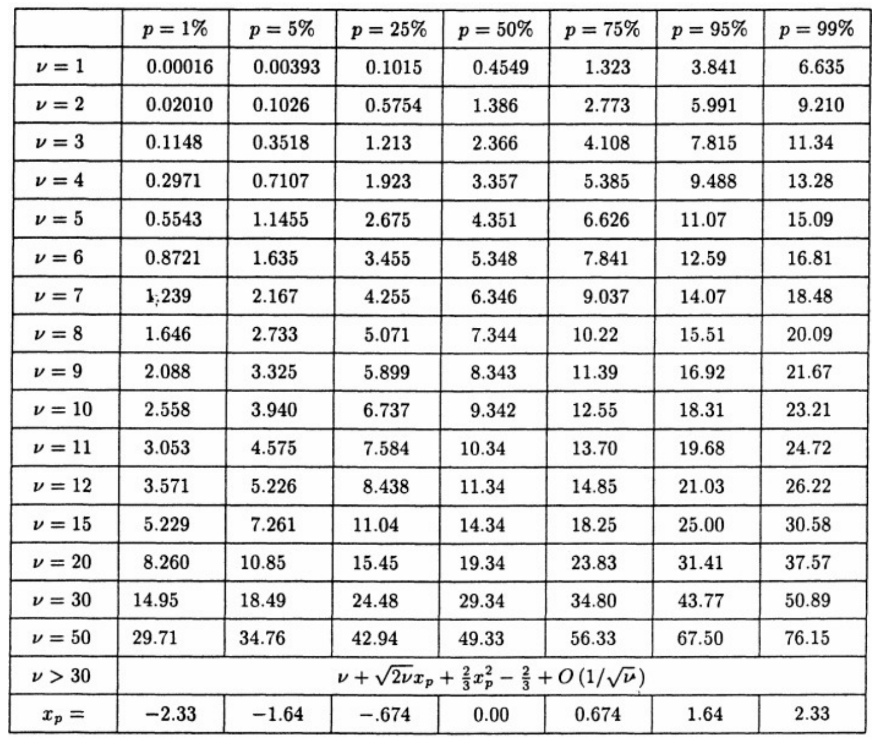
\includegraphics[scale=0.4]{7.jpg}
	\label{fig:screenshot007}
	\caption{Некоторые процентные точки $\chi^2$ - распределения}
\end{figure}

Таким образом, процедура проверки следующая:
\begin{itemize}
    \item Выделяем k категорий. В нашем случае это количество возможных полученных значений: 10, 90 и 900 для одноразрядных, двухразрядных и трехразрядных;
    \item Запускаем генератор случайных чисел N раз;
    \item Определяем количество случайных чисел, попавших в каждую категорию;
    \item Вычисляем значение V по формуле (2);
    \item Сравниваем полученное значение с теоретическими значениями в таблице, определяем к какому интервалу оно относится;
    \item Делаем выводы о случайности величины, возможны три случая:
    \begin{itemize}
        \item Если Vэксп лежит между 1\% и 99\% точками, то генератор удовлетворителен. (Однако необходимо учитывать «подозрительные результаты», о которых написано выше);
        \item Если Vэксп меньше 1\% точки, то генератор не удовлетворителен, так как разброс чисел слишком мал, чтобы быть случайным;
        \item Если Vэксп больше 99\%  точки, то генератор не удовлетворителен, так как разброс чисел слишком велик, чтобы быть случайным.
    \end{itemize}
\end{itemize}



\section*{Результаты работы}

\begin{figure}[H]
	\centering
	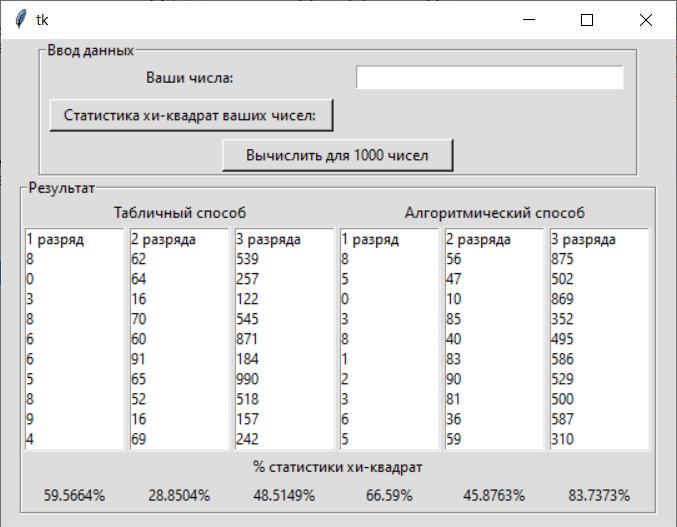
\includegraphics[scale=0.8]{1v.png}
	\label{fig:screenshot001}
\end{figure}

\begin{figure}[H]
	\centering
	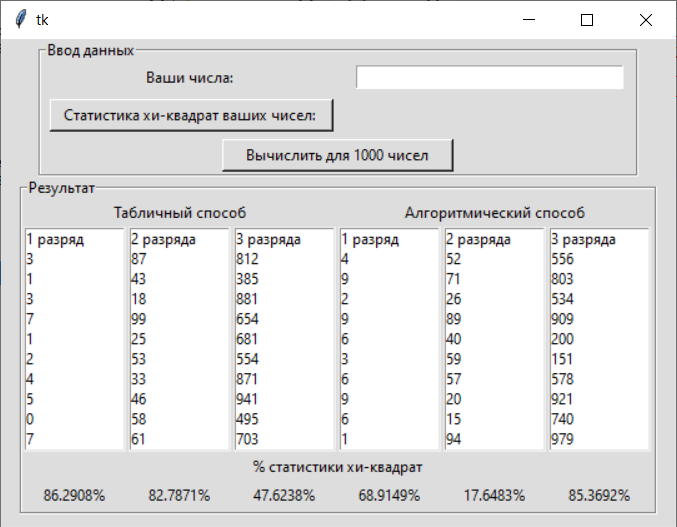
\includegraphics[scale=0.8]{2v.png}
	\label{fig:screenshot002}
\end{figure}

\begin{figure}[H]
	\centering
	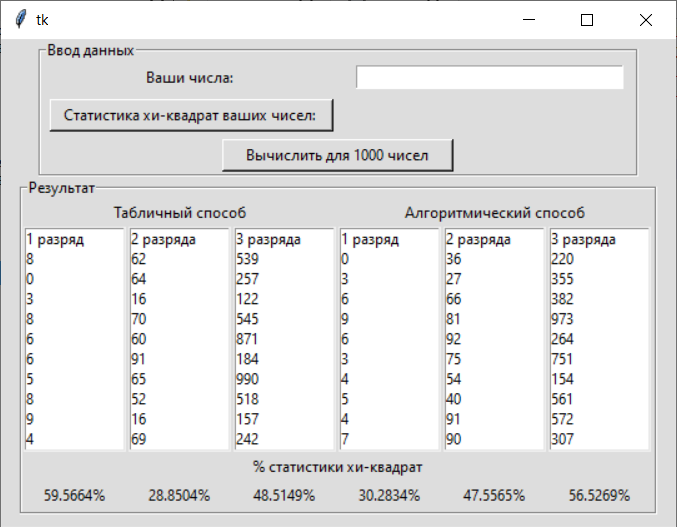
\includegraphics[scale=0.8]{3v.png}
	\label{fig:screenshot003}
\end{figure}

\begin{figure}[H]
	\centering
	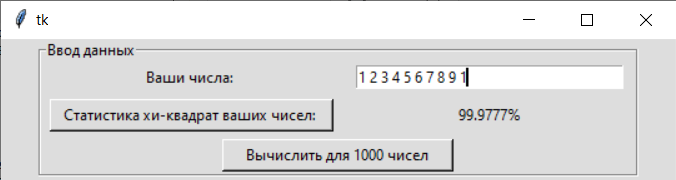
\includegraphics[scale=0.8]{4v.png}
	\label{fig:screenshot004}
\end{figure}

\begin{figure}[H]
	\centering
	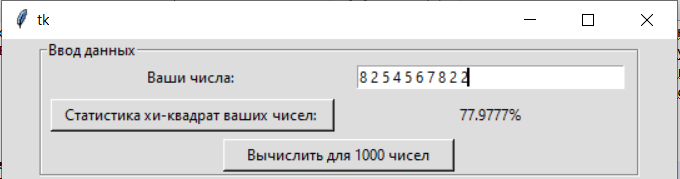
\includegraphics[scale=0.8]{5v.png}
	\label{fig:screenshot005}
\end{figure}

\begin{figure}[H]
	\centering
	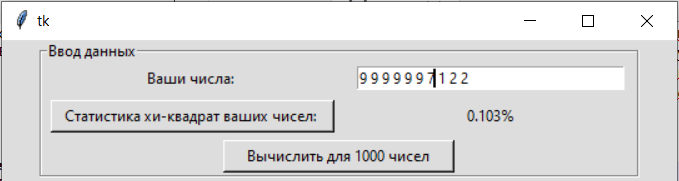
\includegraphics[scale=0.8]{6v.png}
	\label{fig:screenshot006}
\end{figure}


\quad Из результатов можно сделать вывод, что в некоторых случаях при применении обоих методов значения приближаются к «подозрительным», однако это не критично и результаты работы генератора можно признать удовлетворительными.

\clearpage

\end{document}

